\documentclass[a4paper,11pt] {article}
\usepackage[spanish]{babel}
\usepackage[utf8]{inputenc}
\usepackage{caratula}
\usepackage{a4wide}
\usepackage{graphicx}
% \usepackage{dot2texi}
% \usepackage{graphs}

\begin{document}

\titulo{Trabajo Pr\'actico Nro. 2}
\fecha{08/05/2009}
\materia{Algoritmos y Estructuras de Datos III}
\grupo{}
\integrante{Dinota, Mat\'ias}{076/07}{matiasgd@gmail.com}
\integrante{Huel, Federico Ariel}{329/07}{federico.huel@gmail.com}
\integrante{Leveroni, Luciano}{360/07}{lucianolev@gmail.com}
\integrante{Mosteiro, Agust\'in}{125/07}{agustinmosteiro@gmail.com}

\maketitle

\bigskip
\section*{Aclaraciones generales}

Antes de comenzar el an\'alisis de cada ejercicio, cabe mencionar lo siguiente:

\begin{itemize}
 \item La implementaci\'on de los 3 algoritmos se realiz\'o en \textbf{lenguaje Java}, haciendo uso de las librer\'ias est\'andar del mismo.
 \item Para el c\'alculo de tiempo de los algoritmos se utiliz\'o la funci\'on \textbf{nanoTime()} de la clase System de Java. Con el fin de aumentar la precisi\'on de las mediciones, se utiliz\'o el comando \textbf{nice} para darle m\'axima prioridad a la tarea.
 \item El c\'odigo fuente de los algoritmos aqui analizados se encuentran en los archivos \textit{Dengue.java} (Ej 1), \textit{Diamante.java} (Ej 2) y \textit{RedAstor.java} (Ej 3).
 \item El c\'odigo fuente de los programas encargados de hacer uso de los algoritmos y necesarios para compilar las aplicaciones son:
 \begin{itemize}
    \item \underline{Ej 1:} MainDengue.java, Dengue.java e InstanciaDengue.java.
    \item \underline{Ej 2:} MainDiamante.java, Diamante.java, InstanciaDiamante.java.
    \item \underline{Ej 3:} MainRedAstor.java, RedAstor.java, InstanciaRedAstor.java, Arista.java, AristaComparator.java, Dupla.java, DuplaComparator.java.
  \end{itemize}
 \item Para la lectura y escritura de los datos se utilizaron clases provistas por el lenguaje Java. No se har\'a referencia a estos algoritmos ya que no resultan de inter\'es para el trabajo aqui presentado.
 \item Los gr\'aficos se realizaron con \textbf{GNUPlot}. En los casos considerados pertinentes, se utiliz\'o una escala logar\'itmica con el fin de poder visualizar mejor los resultados.
\end{itemize}

\begin{center}
\section*{Ejercicio 1: Dengue}
\end{center}

\bigskip
\section*{Introducci\'on}

El objetivo del siguiente ejercicio es diseñar un algoritmo que resuelva el problema planteado de manera polinomial. Para esto se utiliz\'o la t\'ecnica de progamaci\'on din\'amica, lo que implic\'o la realizaci\'on de diversos pasos. Primero se corrobor\'o que el problema cumpla con el principio de optimalidad. Una vez comprobado esto (condici\'on necesaria para poder aplicar programaci\'on din\'amica) y utilizando las ideas vistas en dicha demostraci\'on, se procedi\'o a crear una funci\'on recursiva que retorne el resultado deseado. Luego se modific\'o dicha version por un algoritmo iterativo, siendo este un paso intermedio requerido para aplicar la t\'ecnica mencionada. El paso siguiente consisti\'o en modificar el algoritmo de manera de evitar la repetici\'on de c\'alculos innecesarios (aqu\'i queda implicita la idea de programaci\'on din\'amica), mejorando notablemente la complejidad de la funci\'on. Por \'ultimo, como veremos m\'as adelante, se opt\'o por un cambio de t\'ecnica algoritmica pasando de un algoritmo que originalmente era \textit{top-down} a uno \textit{bottom-up}.

\section*{Algoritmo}

En la presente secci\'on presentaremos todos los pasos que se siguieron para lograr la implementaci\'on del algoritmo que resuelve el problema. Como se mencion\'o anteriormente, el problema ser\'a resuelto por medio de la t\'ecnica de programaci\'on din\'amica por lo que presentaremos las demostraciones de todos los pasos que implica construir un algoritmo de esa manera. En primer lugar, se demostrar\'a c\'omo aplica el principio de optimalidad en el problema dado. En segundo lugar, plantearemos una funci\'on recursiva que resuelva el problema y demostraremos su correctitud. Finalmente, mostraremos el algoritmo construido con programaci\'on din\'amica, explicando detalladamente por qu\'e resuelve el problema de manera m\'as eficiente que la soluci\'on recursiva.

\subsection*{Principio de optimalidad}

Demostraremos por qu\'e vale el principio de optimilidad en este problema por el absurdo.

Sean $n$ y $l$ la cantidad de zonas y litros disponibles respectivamente y que las zonas se numeran de $1$ a $n$. Suponemos que la cantidad de mosquitos muertos con $l$ litros hasta la zona $n$ es \'optima y llamaremos $P$ a dicha cantidad. Sea $k$ la cantidad de litros usados en la zona $n$, suponemos que hasta la zona $n-1$ usando $l-k$ litros la cantidad de mosquitos muertos ($Q$) no es \'optima y se intenta llegar a un absurdo.

Si hasta la zona $n-1$ la cantidad de mosquitos muertos no es \'optima (para $l-k$ litros), existe otra forma de distribuir los $l-k$ litros entre las zonas $1$ a $n-1$ que hace que la nueva cantidad, a la que llamaremos $R$, sea \'optima (es decir, $R > Q$). Entonces tenemos que

$R + cantMM(n,k) > Q + cantMM(n,k) = P \Rightarrow R + cantMM(n,k) > P$

Esto es un absurdo ya que supusimos que $P$ era la cantidad \'optima. Este absurdo surge de suponer que la cantidad de mosquitos muertos hasta la zona $n-1$ con $l-k$ litros no era \'optima. Entonces queda demostrado que vale el principio de optimalidad para el problema planteado.

\subsection*{Soluci\'on recursiva y demostraci\'on de correctitud} %TODO!!!!!!!!!!!!!!!!!!!!!

A partir de la idea presentada en la secci\'on anterior se puede plantear la siguiente funci\'on recursiva para resolver el problema.
$\\ f(0, l) = 0 \\$
$ f(i,l) = max \left\{ \begin{array}{ll}
         f(i-1,l) & \mbox{$$}\\
        f(i-1, l-k) + MM[i][k] & \mbox{con $1 \leq k \leq l$}\end{array} \right. $


Siendo $MM[i][j]$ la matriz que contiene la cantidad de mosquitos muertos por litro, de cada zona. La soluci\'on al problema ser\'ia $f(n,l)$ con $n$ la cantidad de zonas y $l$ la cantidad de litros disponibles.

Para demostrar que la funci\'on presentada es correcta utilizaremos inducci\'on en la cantidad de zonas manteniendo la cantidad $l$ de litros fija. Es decir, queremos probar la siguiente proposici\'on. \\

P(n): $f(n, i)$ es la cantidad m\'axima de mosquitos muertos hasta la zona $n$ con $i$ litros. ($0 \leq i \leq l$) \\

\textbf{Caso Base ($P(1)$)}

$f(1,i) = max_{0 \leq j \leq i} (MM[1][j]) \;\;\;\; $ con $i \leq 1$

Entonces, como se puede notar, $f(1,i)$ = $f (1,1)$ por lo que es trivialmente la cantidad m\'axima de mosquitos muertos de la primera zona con $i$ litros. \\

\textbf{Paso inductivo ($P(n) \Rightarrow P(n+1)$)}

Supongo que $f(n,i)$ es la m\'axima cantidad de mosquitos muertos hasta la zona $n$ con $i$ litros ($0 \leq i \leq l$) y demuestro que $f(n+1,i)$ es la cantidad m\'axima hasta la zona $n+1$.
Como $n+1 > 1$ tenemos que \\

$f(n+1,i) = max_{0 \leq k \leq i} (f(n, i-k) + MM[n+1][k])$ \\

Como $i - k \leq l$ para cualquier $k \leq i$ puedo aplicar la hip\'otesis inductiva, es decir, $f(n,i-k)$ es la m\'axima cantidad hasta la zona $n$ con $i-k$ litros. Entonces con $max_{0 \leq k \leq i} (f(n, i-k) + MM[n+1][k])$ obtengo la m\'axima cantidad de mosquitos muertos hasta la zona $n+1$ con $i$ litros pues $f(n,i-k)$ es m\'axima y se calcula el m\'aximo para todas las cantidades $k$ de litros posibles para dicha zona. Entonces, como vale $P(1)$ y $P(n) \Rightarrow P(n+1)$ por principio de inducci\'on queda demostrada la proposici\'on.

La funci\'on presentada, a pesar de ser correcta, hace repetidas llamadas recursivas a valores ya calculados. Sin embargo, sirve de base para idear un algoritmo que use la t\'ecnica de programaci\'on din\'amica para resolver este problema de forma m\'as eficiente. En las posteriores secciones veremos en detalle c\'omo se relaciona dicha funci\'on con el algoritmo implementado.

\subsection*{Algoritmo utilizando programaci\'on din\'amica}

A continuaci\'on se encuentra el pseudoc\'odigo del algoritmo que utiliza la t\'ecnica de programaci\'on din\'amica para resolver el problema.

\begin{verbatim}
maxMMParcial[zonas][litros]

lleno la primer fila de maxMMParcial con 0

para i desde 1 hasta zonas
  para j desde 0 hasta litros
    max_parcial = maxMMParcial[i-1,j]
    k = 1
    mientras k <= j
      max_parcial = maximo(max_parcial, maxMMParcial[i-1,j-k] + MM[i][k])
    maxMMParcial[i][j] = max_parcial

\end{verbatim}

% litrosPorZona[zonas]
% 
% litrosRestantes = litros
% j = litrosRestantes
% para i desde zonas hasta 1
%   mientras j >= 0 y (maxMMParcial[i][litrosRestantes] - MM[i-1][litrosRestantes - j]) != maxMMParcial[i-1][j]
%     j = j - 1
%   litrosPorZona[i-1] = litrosRestantes - j
%   litrosRestantes = j

% guardar en Tp2Ej1.out litrosPorZona

Este algoritmo est\'a basado en la funci\'on recursiva presentada en la secci\'on anterior, pero usando una estrategia \textit{Bottom-up} para calcular el resultado. Dicha estrategia se basa en el uso de una matriz para almacenar los resultados ya calculados y, a partir de ellos, construir las distintas etapas de la soluci\'on. Esta matriz tiene la siguiente forma:

\begin{center}
litros
\end{center}
\[ zonas \left( \begin{array}{ccccc}
0 & 0 & 0 & \cdots & 0 \\
0 & f(1,1) & f(1,2) & \cdots & f(1,l)  \\
0 & f(2,1) & f(2,2) & \cdots & f(2,l)	\\
\vdots & \vdots & \vdots & \ddots & \vdots \\
0 & f(n,1) & f(n,2) & \cdots & f(n,l) \end{array} \right)\]

En el algoritmo presentado cada fila de esta matriz se construye a partir de la fila anterior, por lo que la primer fila (que representa el caso base de $f$) debe ser 0 al comienzo del procedimiento. Adem\'as, en este c\'alculo tambi\'en es necesario utilizar los valores de la matriz de entrada (MM) que contiene la cantidad de mosquitos muertos seg\'un la cantidad de zonas y litros.
Esto se corresponde a la definici\'on recursiva de la funci\'on $f$ ya que el valor que retorna $f$ para cada zona $i$ se construye a partir de la zona $i-1$. 

Como se puede apreciar en el pseudoc\'odigo cada elemento de la matriz se construye de la siguiente manera:

$ maxMMParcial[i][j] = max \left\{ \begin{array}{ll}
         maxMMParcial[i-1][j] & \mbox{$$}\\
        maxMMParcial[i-1][j-k] + MM[i][k] & \mbox{con $1 \leq k \leq j$}\end{array} \right. $


Esta definici\'on muestra claramente la relaci\'on que existe entre el algoritmo que utiliza programaci\'on din\'amica y la funci\'on que resuelve el problema de manera recursiva. Cada posici\'on de la matriz se calcula de la misma manera que $f$, por lo que, si el caso base es el mismo, se obtendr\'an los mismos resultados. Por esta raz\'on, al terminar de calcular toda la matriz (hasta la posici\'on $n$ y $l$) se obtiene $f(n,l)$, es decir, la soluci\'on para la instancia del problema.

\subsection*{Cálculo de los litros por zona}

Una vez obtenida la matriz que contiene los valores óptimos para las distintas instancias del problema. Se implementó un algoritmo para utilizar estos valores de manera tal de encontrar la cantidad de litros que debían emplearse en cada zona para finalmente obtener el valor óptimo ya calculado.

Este algoritmo consistió en, utilizando el principio de optimalidad, recorrer la matriz de la última fila hacia la primera, observando cómo cambiaría el valor en la matriz de una zona a otra utilizando una determinada cantidad de litros y cuál fue el cambio observado. Al coincidir el resultado observado con el esperado, se encuentra la cantidad de litros que deben ser utilizados en esa zona y se guarda en un array. Una vez recorridas todas las filas de la matriz, se posee un array con los litros que deben usarse en cada zona para conseguir el resultado óptimo.

\begin{verbatim}
recorrer matriz maxMMparcial desde la ultima fila a la primera
  Buscar en cada fila (i) en MM los listros que cumplan con que:
    maxMMparcial[i][litrosQueNoUse] - los mosquitos muertos en la zona i con esos litros
    = a maxMMparcial[i-1][litrosQueNoUse - litros que acabo de usar].
  guardar en litrosUsadosEn[i] los litros encontrados para dicha zona.
\end{verbatim}

\section*{Complejidad}

En la presente secci\'on se calcular\'a la complejidad en el peor caso del algoritmo \textit{fumigar} bas\'andose en el modelo de c\'omputo uniforme. Esto se debe a que este ejercicio no se basa en el tama\~{n}o de los elementos de la matriz recibida como par\'ametro, sino en las dimensiones de dicha matriz, por lo que no se trabajar\'a con valores muy altos. Para realizar los c\'alculos de manera m\'as clara, se dividir\'a el analisis en el estudio de las dos partes que conforman la funci\'on: \textit{fumigaci\'on} y \textit{c\'alculo de litros por zona}

En la funci\'on \textit{fumigaci\'on} todas las operaciones y asignaciones utilizadas se logran en tiempo constante. Esto se debe al mencionado modelo de c\'omputo utilizado, en donde las operaciones presentes en el algoritmo no dependen del tama\~{n}o de los par\'ametros de entrada. De esta manera, la complejidad de esta funci\'on estar\'a supeditada al comportamiento de los ciclos que contiene. Llamaremos $a$ $b$ y $c$ a los ciclos, donde $a$ contiene a $b$ y este \'ultimo contiene a $c$. Se puede apreciar claramente que b itera $m$ veces (donde $m$ es la cantidad de litros) y que en cada iteraci\'on de b, se realiza una vez el ciclo c. El l\'imite de este ciclo esta dado por la variable de iteraci\'on de b (en el pseudoc\'odigo se llamada $j$), de manera que, en cada iteraci\'on de b, la cantidad de vueltas del ciclo c aumenta en uno, comenzando desde cero (valor de inicio de la variable $j$) hasta $m$. La complejidad del ciclo b sera entonces:

$$\sum_{j=0}^{m}j=\sum_{j=1}^{m}j=(m+1)m/2\ \in O(m^{2})  $$

El ciclo analizado se encuentra dentro de $a$, este \'ultimo se recorre $n$ veces (donde $n$ es la cantidad de zonas) debido a que su variable de iteraci\'on (en el pseudoc\'odigo llamada $i$) es inicializada en cero y aumentada en uno hasta llegar al valor $n$. Finalmente podemos concluir que la complejidad de la funci\'on \textit{fumigaci\'on} es:

$$T(n,m)=n((m+1)m/2)\ \in O(nm^{2})$$

Por otro lado, analizaremos la complejidad en peor caso de la otra parte del algoritmo: \textit{c\'alculo de litros por zona}. En cuanto a los costos de las operaciones matem\'aticas y asignaciones, sucede lo mismo que en el caso anterior por lo que nuevamente el estudio de la complejidad se concentrar\'a en los ciclos. En este caso tenemos dos ciclos. Se puede apreciar facilmente que el ciclo externo realiza $n$ iteraciones ya que la variable $i$ utilizada para iterar es inicializada en $n$ y es decrementada hasta llegar a 1. Como muestra el pseudoc\'odigo, el limite del ciclo interno esta dado por una condici\'on por lo que la cantidad de iteraciones que realize var\'ia cada vez que es ejecutado. Lo que si se puede ver es que, en total (es decir, para las $n$ iteraciones del ciclo externo), el ciclo ser\'a recorrido $m$ veces. Esto se debe a que en caso de cumplir con la condici\'on mencionada, la variable de iteraci\'on del ciclo $j$ es decrementada en 1, y nunca es reiniciada. Como dicha variable es inicializada con la cantidad de litros y en cada vuelta del ciclo interno se corrobora que su valor sea mayor o igual que cero, podemos concluir que dicho ciclo ser\'a recorrido $m$ veces en total (ya que si se cumple la condici\'on, $j$ es decrementado, y si no se satisface la guarda, no se entra al ciclo). Por estos motivos la segunda parte del algoritmo de \textit{fumigar} tiene complejidad $T(n)\ \in O(n+m)$.

De esta manera, como la complejidad de la primer parte de la funci\'on pertenece a $O(nm^{2})$, la segunda pertenece a $O(n+m)$ y $O(n+m)\ \in O(nm^{2})$, concluimos que la complejidad en peor caso del algoritmo \textit{fumigar} es $$T(n,m) \in O(nm^{2})$$

Finalmente estudiaremos la complejidad en funci\'on del tama\~{n}o de la entrada. Sea $t$ el tama\~{n}o de la entrada, $n$, $m$ y $M$ la cantidad de zonas, litros y la matriz pasados como par\'ametros respectivamente. Tenemos entonces que:

$$t=\log(n)+\log(m)+\sum_{i=1}^{n}\sum_{j=1}^{m}\log(M_{i,j})>\log(n)+\log(m)+\sum_{i=1}^{n}\sum_{j=1}^{m}1>\log(n)+\log(m)+nm>nm$$

\hspace{45pt} $\Longrightarrow$ como $T(n,m) \in O(nm^{2})$ y $nm^{2}<(nm)^{2}<t^{2} \Longrightarrow T(t) \in O(t^{2})$

\section*{An\'alisis de resultados}

Con el fin de analizar la complejidad de los algoritmos propuestos (fumigaci\'on y c\'alculo de litros por zona) se realizaron varias pruebas. Estos experimentos est\'an orientados a estudiar el tiempo de ejecuci\'on del mismo en relaci\'on a los datos de entrada, comparando el costo real de los algoritmos junto con su complejidad te\'orica calculada. Para cada algoritmo se ver\'an 3 gr\'aficos distintos. El primero de ellos servir\'a para analizar la complejidad con respecto a los litros, es decir, fijando la cantidad de zonas. Reciprocamente, el segundo ser\'a en base a la cantidad de zonas con una cantidad fija de litros. Por \'ultimo, el tercer gr\'afico en 3 dimensiones mostrar\'a como se comporta el algoritmo considerando ambas variables en conjunto.

A continuaci\'on se describir\'an las caracter\'isticas de las instancias utilizadas para las pruebas as\'i como las particularidades de cada experimento. Dichas cuestiones son comunes al analisis de ambos algoritmos por lo que no haremos referencia a ninguno en particular. M\'as adelante analizaremos resultados de estos experimentos aplicado a cada uno de los algoritmos.

Para las instancias de prueba se utiliz\'o la funci\'on \textit{random} del lenguaje para generar matrices de \textit{mosquitosMuertos}) de tamaño $zonas*litros$ con valores aleatorios comprendidos entre $1$ y $10000$ con el fin de garantizar que las pruebas resulten lo suficientemente gen\'ericas como para poder obtener resultados ``interesantes''. Cabe mencionar que no se har\'an estudios sobre instancias particulares ya que, como se mencion\'o antes, el costo de ejecuci\'on del algoritmo de \textit{fumigaci\'on} no depende de los valores de la matriz de entrada que conforma cada instancia.

En primer lugar, se hicieron c\'alculos utilizando como variable la cantidad de zonas a fumigar, fijando en $10$ los litros disponibles. El rango de zonas analizados es desde $1$ hasta $10000$ zonas, de a intervalos de tamaño $10$. La elecci\'on de estos valores fue producto del an\'alisis de 2 cuestiones importantes: que n\'umeros permitir\'ian tomar muestras utiles para la realizaci\'on de los gr\'aficos y cual era la m\'axima cantidad de datos que nuestra aplicaci\'on podr\'ia manejar, acotada por el tiempo disponible para realizar las pruebas y las limitacion propias de la m\'aquina en cuesti\'on. Empiricamente, se comprob\'o que dicho rango de zonas permit\'ia correr la aplicaci\'on en un tiempo razonable y al mismo tiempo proveer datos interesantes para el an\'alisis en cuesti\'on. Del mismo modo, fijar en 10 los litros asegur\'o que sea la cantidad de zonas el par\'ametro ponderante en el c\'alculo de tiempo de ejecuci\'on.

La segunda prueba resulta muy similar a la anterior en cuanto al rango de valores utilizados. La diferencia radica en que ahora el par\'ametro fijado es la cantidad de zonas en vez de la cantidad de litros, variando los litros en el rango $1$ hasta $10000$, de a intervalos de tamaño $10$ (al igual que en la prueba anterior).

La tercer y \'ultima prueba consisti\'o en analizar el algoritmo considerando ambas variables en conjunto, de modo de poder comparar el tiempo de ejecuci\'on para distintos valores de zonas y litros junto con la complejidad te\'orica que depende de estos dos par\'ametros. Para esta prueba se tomaron valores de zonas y litros entre $1$ y $1000$, de a intervalos de tamaño $100$ (10 valores posibles). Luego, se calcularon los tiempos de ejecuci\'on de todas las permutaciones de los 10 elementos pertenecientes a dicho conjunto de manera tal de obtener resultados para las combinaciones de litros y zonas dentro del intervalo mencionado.

A continuaci\'on se presentar\'an los gr\'aficos realizados para cada algoritmo utilizando estas 3 pruebas descriptas.

\subsection*{Fumigaci\'on}

Como se vi\'o anteriormente, la primer parte del problema consist\'ia en calcular la m\'axima cantidad de mosquitos muertos para una instancia determinada. Los siguientes gr\'aficos muestran el comportamiento de este algoritmo en base a los dos par\'ametros de entrada de manera independiente:

\begin{center}
 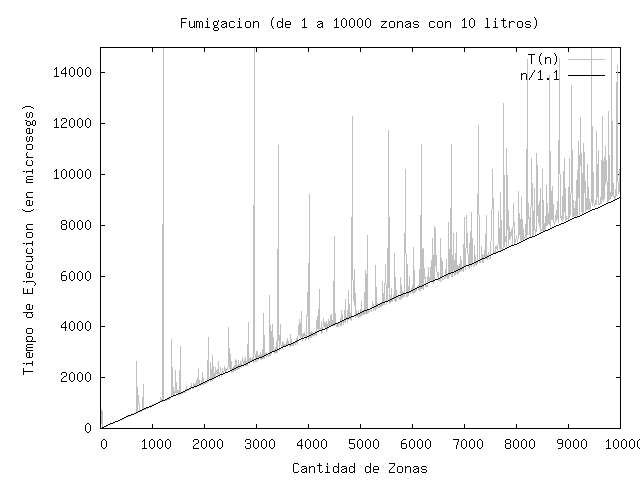
\includegraphics[width=0.7\textwidth]{Plots/Tp2Ej1-TiemposFumigacionPorZonas-10litros-bw.png}
\begin{center}
Figura 1.1
\end{center}
 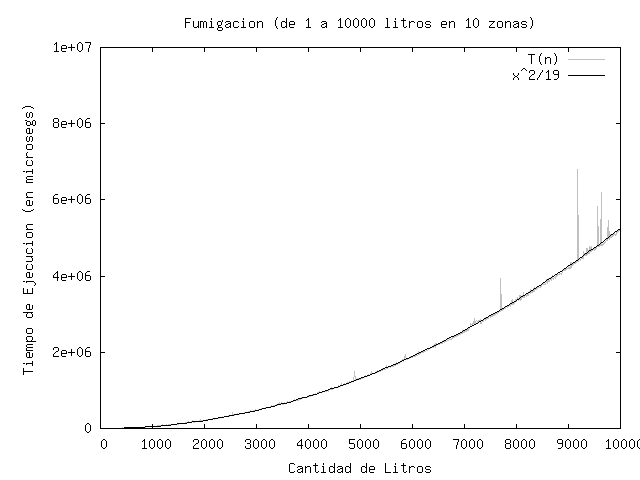
\includegraphics[width=0.7\textwidth]{Plots/Tp2Ej1-TiemposFumigacionPorLitros-10zonas-bw.png}
\begin{center}
Figura 1.2
\end{center}
\end{center}

Ambos gr\'aficos permiten observar algunas cuestiones interesantes. La Figura 1.1 permite observar como el comportamiento del algoritmo de \textit{fumigaci\'on} con respecto a la cantidad de zonas se asimila a una funci\'on lineal, hecho que se corresponde con la complejidad calculada anteriormente. Del mismo modo, la Figura 1.2 muestra como la funci\'on T(n) que representa el tiempo de ejecuci\'on se comporta pr\'acticamente igual que la funci\'on $f(n) = n^2/19 \in O(n^2)$. Este hecho demuestra emp\'iricamente que la complejidad con respecto a la cantidad de litros es cuadr\'atica al realizar la fumigaci\'on tal como se hab\'ia analizado anteriormente.

Otras cuesti\'on observable son los ``picos'' y variaciones abrutas en ambos gr\'aficos. En principio, esto no deber\'ia ocurrir ya que la complejidad no depende de la forma de la entrada como se mencion\'o anteriormente. El motivo de esto radica simplemente en los errores de precisi\'on en la medici\'on de las operaciones propios de las limitaciones de la m\'aquina de c\'omputo utilizada. Los tiempos de ejecuci\'on del algoritmo son mucho mayores en la Figura 1.2 lo que resulta en una mayor estabilidad en los c\'alculo de tiempo, en contraste con la Figura 1.1 donde hay mayor impresici\'on porque dicho gr\'afico refleja cambios de valores m\'as abrutos.

\begin{center}
 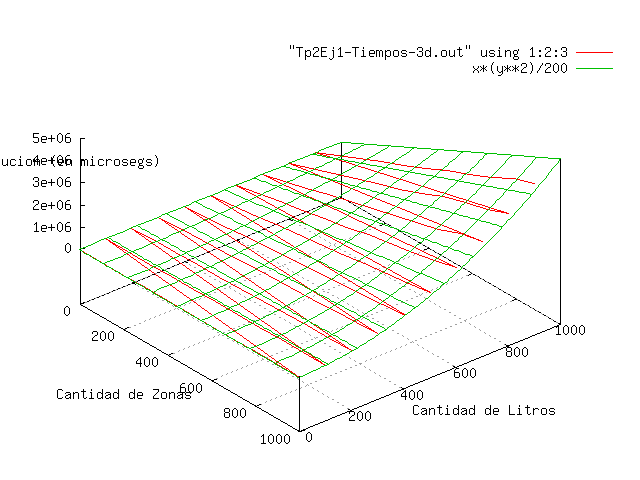
\includegraphics[width=0.7\textwidth]{Plots/Tp2Ej1-TiemposFumigacion-3d-bw.png}
\begin{center}
Figura 1.3
\end{center}
\end{center}

Esta \'ultima figura permite ver como el algoritmo en su totalidad realmente se comporta de la forma esperada. 
Para esto basta comparar los tiempos de ejecuci\'on al variar ambos par\'ametros (litros y zonas) junto con la funci\'on $f(n,m) = n*m^2/200 \in O(n*m^2)$ viendo que ambas ``mantas'' coiniciden. Este ultimo hecho constituye la \'ultima prueba de que empir\'icamente el algoritmo funciona tal como se esperaba.

\subsection*{C\'alculo de Litros Por Zona}

En esta secci\'on analizaremos el comportamiento del otro algortimo propuesto que se encarga de dar parte de la soluci\'on del problema: el algoritmo encargado de calcular los litros a utilizar por cada zona. Los siguientes gr\'aficos muestran el comportamiento del mismo en base a las dos variables en cuesti\'on de forma independiente:

\begin{center}
 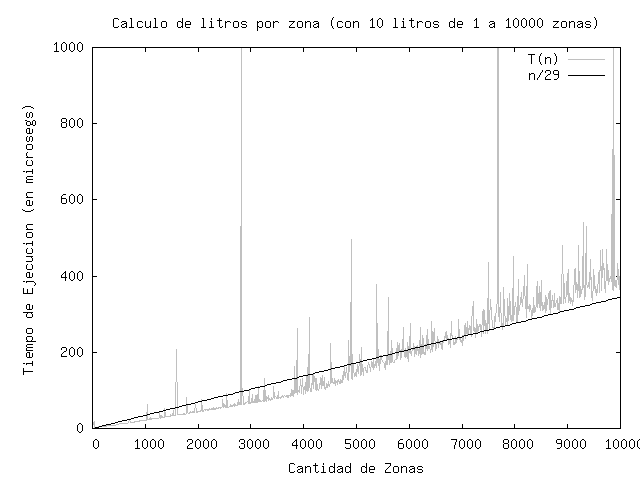
\includegraphics[width=0.7\textwidth]{Plots/Tp2Ej1-TiemposLitrosPorZonaPorZonas-10litros-bw.png}
\begin{center}
Figura 2.1
\end{center}
 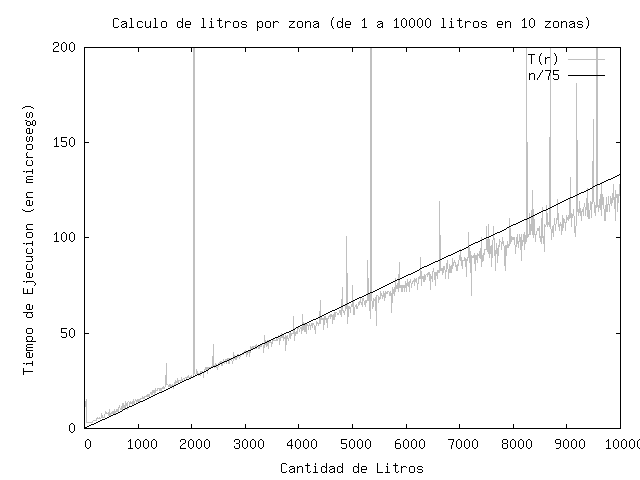
\includegraphics[width=0.7\textwidth]{Plots/Tp2Ej1-TiemposLitrosPorZonaPorZonas-10zonas-bw.png}
\begin{center}
Figura 2.2
\end{center}
\end{center}

Como se puede observar, en ambos casos, el comportamiento del algoritmo es el esperado. La Figura 2.1 muestra como el c\'alculo de litros por zona se ``corresponde'' con el gr\'afico de la funci\'on lineal $f(n) = n/25$ al variar la cantidad de zonas y fijar los litros en $10$. As\'imismo, la Figura 2.2 se comporta de la forma $f(n) = n/75$ al variar los litros y fijar las zonas. Esto comprueba la linealidad en complejidad te\'orica analizada previamente para ambas variables. Un punto interesante a observar es que las constantes que acompañan a estas funciones difieren, siendo la constante relacionada al primer gr\'afico ($1/25$) 3 veces mayor que la otra ($1/75$). Al tratarse de instancias de igual tamaño (en ambos casos, matrices desde $1*10$ hasta $10000*10$), se puede concluir que la \textit{performance} de este algoritmo depende en mayor medida de la cantidad de zonas que de la cantidad de litros. En otras palabras, para instancias de igual tamaño, un caso demora 3 veces m\'as el otro. Si bien se intentó buscar una explicación a este fenómeno, se concluyó que resulta muy complejo observar cual es la causa de esta particularidad, principalmente porque se está trabajando con instancias aleatorias con parámetros arbitrarios.

Con respecto a la irregularidad del gr\'afico, cabe notar que, a diferencia del algoritmo anterior, este algoritmo no realiza siempre la misma cantidad de operaciones para instancias de igual tamaño tal como se vi\'o en la secci\'on de an\'alisis de complejidad, ya que el recorrido inverso de la matriz resultante depende justamente de los valores que esta contenga que dependen a su vez de los valores de la matriz de entrada \textit{mosquitosMuertos} (ver secci\'on \textit{Algoritmo}). Por este motivo, debido a que se trata de instancias aleatorias, es esperable que no se obtenga un comportamiento ``tan'' similar a la funci\'on lineal propuesta como ocurre para el primer algoritmo.

Por \'ultimo, al igual que para el algoritmo anterior, se presenta el siguiente gr\'afico de 3 dimensiones:

\begin{center}
 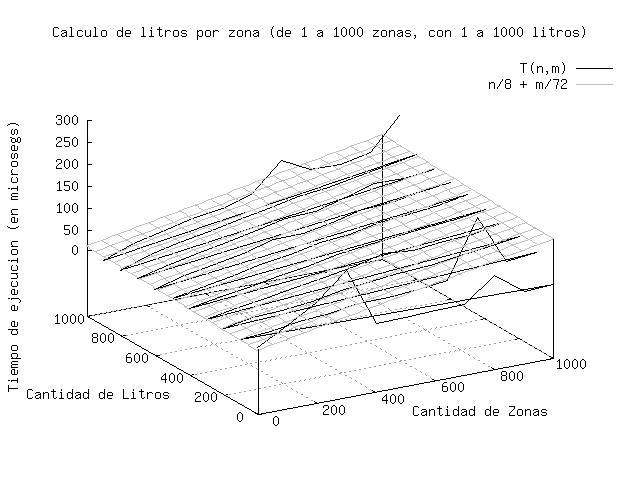
\includegraphics[width=0.7\textwidth]{Plots/Tp2Ej1-TiemposLitrosPorZona-3d-bw.png}
\begin{center}
Figura 1.3
\end{center}
\end{center}

Al igual que antes, este gr\'afico permite ver la complejidad de ambos par\'ametros en conjunto. Cabe notar al tratarse de un algorimto más veloz que el primer caso, los errores de cálculo de tiempo son aún mayores por lo cual no resulta simple obtener una conclusión demasiado fiable. Sin embargo, se puede ver que la función $f(n,m) = n/8 + m/72 \in O(n + m)$ resulta una estimación aceptable para $T(n,m)$. Al igual que antes, podemos concluir que la complejidad teórica total del algoritmo calculada tiene directa relación con los resultados obtenidos.

\section*{Conclusiones}

Este ejercicio srivió fundamentalmente para descubrir y profundizar las caracteríticas principales de la programación dinómica.
Los aspectos más relevantes estudiados fueron la comparación en complejidad y dificultad de implementación entre un algoritmo que actúa de manera ingenua y otro que utiliza la técnica de programacién dinámica y lo determinante que es la utilización del principio de optimalidad en este tipo de ejercicios.

En términos de complejidad, el algoritmo tiene una gran eficiencia respecto de su 'competidor'. Claro está que el algoritmo recursivo con el que fue comparado no propone ningún tipo de eficiencia, no obstante es el más natural de imaginarse, lo que también muestra cómo puede optimizarse un algoritmo con complejidad exponencial a otro polinomial utilizando alguna técnica algorítmica aplicable.

Si bien la función recursiva utilizada mostró gran deficiencia, sirvió para tener la idea del algoritmo y a partir de ella, comenzar a pensar en còmo aplicar programación dinámica.

Respecto de la dificultad de la implementación, quedò absolutamente claro que la solución recursiva era intuitiva y sencilla mientras que el algoritmo de programación dinámica requiere de un pensamiento más elavorado. Sin embargo, el ejercicio mostró que entendiendo como aplica el principio de optimalidad al problema, las ideas se vuelven mucho más claras y menos desagradables.
En un comienzo el principio de optimalidad parecía sencillo de entender. Sirvió para construir una matriz que guardara los valores óptimos hasta el momento que eran usados para calcular los siguientes. Una vez obtenido el resultado óptimo para el problema planteado, empezó la parte rebuscada del uso del principio de optimalidad, pero también la más interesante.

No fue para nada sencillo ver como usar los valores calculados, y el principio para calcular los litros que debían emplearse en cada zona para obtener el mejor resultado. Ésta fue la parte más complicada del algoritmo, comprender cómo volver por la matriz para obtener los datos deseados que nos interesaban.

En este punto fue donde el principio de optimalidad necesitó ser realmente comprendido y mostró su importancia en el algoritmo de programación dinámica.

Desde el punto de vista de la demostración también resulta crucial tener claro el principio de optimalidad y demostrarlo ya que en este se basa la programación dinámica. El ejercicio mostrò una relaciòn entre el principio de optimalidad y la posibilidad de la utilizaciòn de inducción para la demostración del algoritmo. Debido a su característica, y teniendo en cuenta que la técnica la utiliza para llegar a la solución, se vuelve natural pensar en partir de un caso base y luego mostrar que se mantiene su correctitud cuando se calcula un valor posterior.

En general, podemos afirmar que los algoritmos de programación dinámica pueden mejorar muchísimo la complejidad sobre otros algoritmos que utilizan otro tipo de técnicas, sin resultar excesivamente complicados. Esa dificultad pasa principalmente por comprender a fondo como aplica el principio de optimalidad en dicho problema y que además, una vez logrado esto, la demostración de correctitud se puede volver màs sencilla.

\bigskip

\begin{center}
\section*{Ejercicio 2: Diamante}
\end{center}

\bigskip
\section*{Introducci\'on}

El objetivo del siguiente ejercicio es dise\~{n}ar un algoritmo que, dado un grafo, encuentre el menor subgrafo inducido isomorfo a un diamante, en caso de que \'este exista. Un diamante puede definirse como un grafo $K_{4}$ menos una arista. Este algoritmo est\'a basado en una propiedad sobre diamantes (enunciada en el Anexo A) que, adem\'as de ser usada para resolver el problema, ser\'a demostrada de manera formal.

En un principio, cuando se comenz\'o a idear el algoritmo, surgi\'o la idea de utilizar solamente la propiedad enunciada para resolver el problema. Es decir, para toda vecindad de cada nodo, estudiar cada componente conexa para determinar si la misma es completa. Sin embargo, esto s\'olo aportaba informaci\'on sobre las componentes conexas que formaban un diamante, pero no brindaba detalles sobre los nodos que formaban el diamante, y no aseguraba que este fuera m\'inimo para dicha componente conexa. Por esta raz\'on, se opt\'o por utilizar un m\'etodo m\'as complejo que, aunque se basa en la propiedad mencionada, obtiene de cada componente conexa no completa (existe diamante) los nodos m\'inimos que forman un diamante. Esto se realiza calculando el m\'inimo nodo que puede formar un diamante y, a partir de este, construir el m\'inimo probando las posibles combinaciones que construyan un diamante. De esta manera se pueden obtener los diamantes m\'inimos de cada componente conexa no completa de una determinada vecindad y as\'i determinar el m\'inimo de la misma. Finalmente, se comparan los diamantes obtenidos de cada vecindad para obtener el m\'inimo diamante del grafo. Este algoritmo ser\'a explicado en detalle, se mostrar\'a su correctitud y se presentar\'a la implementaci\'on y pruebas de ejecuci\'on del mismo en posteriores secciones.

\section*{Demostraci\'on de la parte a}

A continuaci\'on se presentar\'a la demostraci\'on de la siguiente propiedad:

Sea $G$ un grafo de $n$ v\'ertices y $m$ aristas, $G$ no contiene un subgrafo diamante como subgrafo inducido si y solamente si para todo v\'ertice $v$, su vecindad $N(v)$ se divide en componentes conexas completas.

Llamaremos $p$ a la proposici\'on ``$G$ no contiene un subgrafo diamante como subgrafo inducido`` y $q$ a la proposici\'on ''para todo v\'ertice $v$, su vecindad $N(v)$ se divide en componentes conexas completas``. Dividiremos la demostraci\'on en dos partes: la implicaci\'on y la rec\'iproca.

\begin{itemize}
\item $p \Longrightarrow q$

Por propiedades de la l\'ogica $p \Longrightarrow q$ equivale a mostrar $-q \Longrightarrow -p$. De esta manera, probaremos aqu\'i que si existe un v\'ertice $v$ tal que su vecindad $N(v)$ contiene una componente conexa no completa entonces $G$ contiene un subgrafo diamante como subgrafo inducido.

Primero probaremos la siguiente propiedad (propiedad 1): Sea $v$ un v\'ertice de $G$ y sea $N(v)$ su vecindad asociada. Si $N(v)$ tiene a $K_{3}$ menos una arista (lo llamaremos $K_{3}-1$) como subgrafo inducido, entonces $G$ contiene un diamante como subgrafo inducido.

Esto se debe a que, al pertenecer $K_{3}-1$ a la vecindad de $v$, el grafo original contiene a $K_{3}-1$ uniendo todos sus vertices con $v$, esto implica agregarle un nodo ($v$) y tres aristas (ya que $v$ es adyacente a los tres nodos que conforman el $K_{3}-1$ porque pertenecen a su vecindad). Como $K_{3}-1$ tiene dos aristas entonces agregando un nodo y sumando tres aristas tengo un $K_{4}-1$ (definici\'on de diamante).

Viendo esto, basta probar que si existe un v\'ertice $v$ tal que su vecindad $N(v)$ tiene una componente conexa no completa entonces dicha componente contiene un $K_{3}-1$. Para esto, mostraremos ahora que todo grafo $G$ conexo y no completo contiene un $K_{3}-1$ (propiedad 2).

Como $G$ no es completo pero si conexo, existen dos nodos $a$ y $z$ tal que no son adyacentes y existe un camino entre ellos. Sea $b$ un nodo adyacente a $a$ que pertenece al camino entre $a$ y $z$. $b$ es distinto de $z$ ya que si fueran iguales $a$ y $z$ ser\'ian adyacentes y eso es absurdo por hipotesis. Ahora tomamos un nodo adyacente a $b$ que tambi\'en pertenezca al camino entre $a$ y $z$ al que llamaremos $c$. Este nodo puede ser igual a $z$ (en caso de que el camino tenga longitud dos) o un nodo intermedio en el camino entre $a$ y $z$. Si $c$ es igual a $z$ entonces me puedo formar un $K_{3}-1$ ya que $a$ es adyacente a $b$, $b$ es adyacente a $z$ y $z$ no es adyacente a $a$ por hipotesis:
\begin{center}
 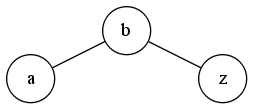
\includegraphics[width=0.34\textwidth]{Grafos/ej2figura1-1.png}
\end{center}
Si $c$ es distinto de $z$ entonces tenemos dos casos: si $c$ no es adyacente a $a$ entonces podemos formar un $K_{3}-1$ con dichos nodos:
\begin{center}
 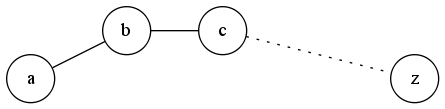
\includegraphics[width=0.6\textwidth]{Grafos/ej2figura1-2.png}
\end{center}
Si $c$ si es adyacente a $a$, entonces no podemos formar un $K_{3}-1$ entre $a$ $b$ y $c$:
\begin{center}
 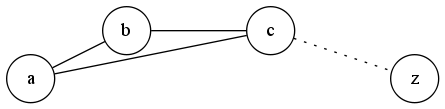
\includegraphics[width=0.6\textwidth]{Grafos/ej2figura1-3.png}
\end{center}
En este \'ultimo caso tomamos como nuevo nodo $b$ a $c$ (es adyacente a $a$ y pertenece al camino entre $a$ y $z$) y como nuevo nodo $c$ a un nodo adyacente a $c$ que pertenezca al camino entre $a$ y $z$ y todavia no haya sido recorrido (siguiendo el orden alfabetico seria el nodo $d$). Nuevamente caemos en el caso anterior, donde la posibilidad de poder armar un $K_{3}-1$ depende de si $d$ es adyacente o no a $a$. Si no es posible obtener un $K_{3}-1$ con el nodo $d$ (debido a que $d$ es adyacente a $a$), seguiremos avanzando los dos nodos pertenecientes al camino entre $a$ y $z$ hasta llegar a que el primero de los dos es el nodo anterior a $z$ (lo llamaremos $y$) del camino y el segundo nodo es igual a $z$. En este caso, siempre es posible armar un $K_{3}-1$ ya que $z$ no es adyacente a $a$ por hipotesis:
\begin{center}
 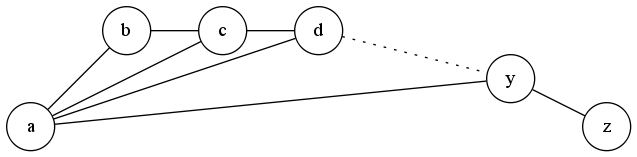
\includegraphics[width=0.85\textwidth]{Grafos/ej2figura1-4.png}
\end{center}
Finalmente hemos probado que si existe un v\'ertice $v$ de $G$ tal que su vecindad $N(v)$ tiene una componente conexa no completa entonces dicha componente contiene un $K_{3}-1$ (por 2), y esto implica que $G$ contiene un subgrafo diamante como subgrafo inducido (por 1).

\item $q \Longrightarrow p$

Por propiedades de la l\'ogica $q \Longrightarrow p$ equivale a mostrar $-p \Longrightarrow -q$. De esta manera, probaremos aqu\'i que si $G$ contiene un subgrafo diamante como subgrafo inducido entonces existe un v\'ertice $v$ tal que su vecindad $N(v)$ contiene una componente conexa no completa.

Sea $G$ un grafo que contiene un subgrafo diamante como subgrafo inducido. Sea $G_{D}$ el subgrafo diamante de $G$:
\begin{center}
 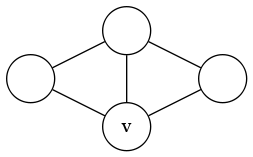
\includegraphics[width=0.34\textwidth]{Grafos/ej2figura2-1.png}
\end{center}
Si tomo uno de los dos nodos de $G_{D}$ de grado tres, que llamaremos $v$, su vecindad $N_{G_{D}}(v)$ sera:
\begin{center}
 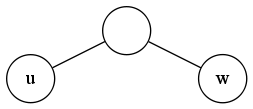
\includegraphics[width=0.34\textwidth]{Grafos/ej2figura2-2.png}
\end{center}
Podemos ver entonces que $N_{G_{D}}(v)$ tiene una \'unica componente conexa y esta no es completa ya que los dos nodos de grado dos del diamante (en la figura llamados $u$ y $w$) no son adyacentes.

Sea $v$ uno de los dos nodos de grado tres del subgrafo diamante de $G$ y $u$ y $w$ los dos nodos de grado dos de dicho diamante. Si tomo la vecindad $N(v)$ de $v$, como $u$ y $w$ son adyacentes a $v$ (pertenecen al diamante) entonces pertenecen a $N(v)$. Ademas como $u$ y $w$ son los nodos de grado dos del subgrafo diamante entonces no son adyacentes en $G$. Como $u$ y $w$ no son adyacentes en $G$ tampoco lo ser\'an para ningun subgrafo inducido de $G$, en particular para $N(v)$. De esta manera la componente conexa de $N(v)$ que contiene al diamante no es completa.

Concluimos entonces que la propiedad es cierta ya que existe un $v$ para el cual se cumple.

\end{itemize}

\section*{Algoritmo}

A continuaci\'on se presenta el pseudoc\'odigo del algoritmo para resolver el problema propuesto.

\begin{verbatim}
crear grafo representado por array de lista de adyacencias (llamado 'adyacencias')
excepto para los nodos de grado 1 y 0

armar la matriz de adyacencias de ese grafo

para cada nodo (que llamaremos superNodo) del grafo
  si el tamaño de la lista de adyacencia de superNodo es mayor que 3
    crear la vecindad del superNodo (crearVecindad)
    buscar el diamante minimo de esa vecindad (buscarDiamanteMinimoEnVecindad)
    y agregarlo a diamantesMinimos (si es que hay alguno)

  si hay algun diamante en diamantesMinimos retorno minimo(diamantesMinimos)

crearVecindad(superNodo)
  para cada nodo k de adyacencias[superNodo]
    para cada nodo j de adyacencias[k]
      si nodo j es adyacente a superNodo
        agregar nodo j a listaVecindad
    vecindadDeSuperNodo[k] = listaVecindad
  devolver vecindadDeSuperNodo (grafo representado por array de listas de adyacencia)

buscarDiamanteMinimoEnVecindad(vecindadDeSuperNodo)
  recorrer cada componente conexa de vecindadDeSuperNodo por DFS
  sumando los grados de los nodos recorridos (sumaGradosCompConexa) y
  guardando en nodosCompConexa los nodos recorridos y
  en nodoMinimoCompConexa el nodo minimo de la componente conexa

  si sumaGradosCompConexa != a la cantidad de nodos
  del grafo completo de los nodos de la comp conexa
    si diamanteMinimo no existe
      diamanteMinimo = diamante minimo de comp conexa actual 
      (buscarDiamanteMinimoDeCompConexa)
    sino
      si nodoMinimoCompConexa <= el minimo nodo de diamanteMinimo
        diamante = diamante minimo de comp conexa actual 
        (buscarDiamanteMinimoDeCompConexa)
        si diamante existe y es mas chico que diamanteMinimo
          diamanteMinimo es ese diamente

  devolver diamanteMinimo (puede ser nulo en caso de que no haya diamante)

buscarDiamanteMinimoDeCompConexa(superNodo, vecindadDeSuperNodo, nodosCompConexa)
  nodo1 = superNodo
  nodoMinimo = nodo minimo de nodosCompConexa con grado menor 
  que cantidad de nodos de la componente conexa - 1

  tuplaMin = <nodo mas grande del grafo, nodo mas grande del grafo>
  para cada nodo (adyacenteANodo2) de vecindadDeSuperNodo[nodo2]
    para cada nodo (nodoCandidato) de vecindadDeSuperNodo[adyacenteANodo2]
      si nodoCandidato no es adyacente a nodo2 
      y <nodoCandidato, adyacenteANodo2> < tuplaMin
        tuplaMin = <nodoCandidato, adyacenteANodo2>

  nodo3 = primero(tuplaMin)
  nodo4 = segundo(tuplaMin)

  diamanteMinimo = ordenar(nodo1, nodo2, nodo3, nodo4)

  devuelvo diamanteMinimo

\end{verbatim}

Como se mencion\'o anteriormente, este algoritmo est\'a basado en la propiedad demostrada en el punto a, es decir, para cada nodo del grafo estudia las componentes conexas de la vecindad de dicho nodo para determinar si existe un diamante. 
El primer paso del algoritmo consiste en cargar las listas de adyacencias provistas en el archivo de entrada a un estructura que llamada \textit{adyacencias}, que no es más que un arreglo de estas listas, donde cada posicion $i$ está asociada a un nodo $i$. Luego, se eliminan todos los nodos de grado 0 \'o 1, ya que estos no pueden formar parte de ning\'un diamante y eliminarlos no afecta a ning\'un diamante del grafo. Esto se debe a que cualquier nodo que pertenezca a un diamante tiene por lo menos grado 2. Para poder eliminar los nodos y poder reducir efectivamente el tamaño del grafo se realizó el siguiente prodecimiento: se creo un nuevo arreglo de adyacencias del tamaño del nuevo grafo (previamente se contaron la cantidad de nodos de grado mayor a 2) y, mediante el uso de arreglos, se realizó un mapeo entre los nodos del grafo original y los valores de los nodos del nuevo grafo para mantener la coherencia de la estructura. Como se observa en el pseudocódigo, al retornar el diamante en cuestión, se realiza un mapeo inverso restaurando los valores de los nodos originales, manteniendo así la consistencia de la entrada de los nodos de entrada. Por último, se creará la matriz de adyacencia que resultar\'a necesaria verificar si dos nodos son adyacentes en tiempo constante (como veremos mas adelante, condición necesaria para cumplir con los requisitos de complejidad).

Luego, el algoritmo comienza a chequear por cada nodo (en adelante llamaremos \textit{superNodo}) su vecindad para encontrar componentes conexas no completas y as\'i determinar donde se encuentra el diamante. La funci\'on \textit{crearVecindad} se encarga de construir la vecindad (que es un grafo representado con una lista de adyacencia) de cada \textit{superNodo} a partir de la lista \textit{adyacencias}, es decir, por cada elemento $k$ de la lista de adyacencia de \textit{superNodo} se recorre la lista de adyacencia del elemento k agregando en la vecindad los elementos que est\'an relacionados con \textit{superNodo}.

Una vez obtenida la vecindad (\textit{vecindadDeSuperNodo}), se comienza a revisar las componentes conexas de la misma para verificar si son completas a trav\'es de la funci\'on \textit{buscarDiamanteMinimoEnVecindad}. Con este fin, se utiliza la técnica \textit{Depth First Search (DFS)} para recorrer cada componente conexa almacenando la suma de los grados de cada nodo recorrido as\'i como el nodo m\'inimo encontrado (\textit{nodoMinimoCompConexa}) y la lista de nodos por los que se avanz\'o (\textit{nodosCompConexa}). Al terminar de recorrer cada componente conexa, se verifica si la misma es completa o no. En caso de que lo sea, se sabe que ninguno de los nodos de esa componente conexa forma un diamante\footnotemark[1], por lo que se descarta y contin\'ua verificando las siguientes componentes. En caso contrario, se procede a encontrar los nodos que forman el diamante\footnotemark[1] m\'inimo para esa componente conexa por medio de la funci\'on \textit{buscarDiamanteMinimoDeCompConexa}. Esta funci\'on busca primero el nodo m\'inimo de la componente conexa que posea grado menor a $n-1$ siendo $n$ la cantidad de nodos de esa componente conexa (identificado como \textit{nodo2}). Luego, toma la lista de adyacencia de ese \textit{nodo2} y para cada nodo $k$ de dicha lista, recorre todos los elementos $j$ de su lista de adyacencia para determinar si forma un grafo $K_{3}-1$ entre \textit{nodo2}, $k$ y $j$ . En este caso, se sabe que los elementos encontrados (\textit{nodo3} y \textit{nodo4}) forman un diamante con \textit{superNodo} (\textit{nodo1}), ya que \textit{superNodo} es adyacente a los mismos pues pertenecen a su vecindad. Como la funci\'on \textit{buscarDiamanteMinimoDeCompConexa} verifica en cada paso si el diamante obtenido es menor al que se tiene hasta ese momento y se prueban todas las posibles diamantes constru\'idos a partir de \textit{nodo2}, se puede afirmar que obtiene el diamante m\'inimo para dicha componente conexa. Esto se debe a que \textit{nodo2} es el menor nodo que puede formar un diamante\footnotemark[1] y los restantes nodos (\textit{nodo3} y \textit{nodo4}) se obtienen seleccionando el menor de todos los posibles diamantes.

Luego, dentro de la funci\'on \textit{buscarDiamanteMinimoEnVecindad} se verifica si el diamante m\'inimo de la componente conexa actual es menor que el diamante que se tiene hasta ese paso (almacenado en \textit{diamanteMinimo}). Si esto sucede, el diamante de la componente conexa actual pasa a ser el diamante m\'inimo. Una vez verificadas todas las componentes conexas se obtiene, en \textit{diamanteMinimo}, el m\'inimo diamante para la vecindad de \textit{superNodo}. Este diamante se almacena en una lista llamada \textit{diamantesMinimos} que, cuando el algoritmo termina de verificar las vecindades de todos los nodos, contendr\'a los diamantes m\'inimos para cada una de las mismas, en caso de que este exista. Finalmente, se busca el m\'inimo de la lista diamantesMinimos, con lo que se obtiene el diamante m\'inimo de todo el grafo, resolviendo as\'i el problema.

\footnotetext[1]{Las demostraciones de estas propiedades fueron presentadas en la secci\'on ``Demostraci\'on de la parte a''}

\section*{Complejidad}

Para calcular la complejidad de este ejercicio el modelo utilizado fue el uniforme, esto se debe a que lo que define el orden del algoritmo es la cantidad de nodos y de aristas
(y cómo están relacionados los nodos  por dichas aristas). Teniendo en cuenta que los nodos van de 1 a $n$, no es relevante observar el tamaño que ocupa cada nodo, sino la cantidad de estos, ya que si el número que representa a un nodo es muy grande, igual de grande es la cantidad de nodos en el grafo y pierde sentido utilizar el modelo logarítmico.

\bigskip
Al crear las listas de adyacencias, el algoritmo lee $2m$ aristas del archivo de entrada y las agrega en dichas listas.  Para esto crea n listas que representan las adyacencias de cada nodo. Como hay $2m$ aristas que se distribuirán en n listas(dónde la inserción es en O(1)), la complejidad temporal de realizar esta tarea será O($2m + n$).
Luego se filtran los nodos de grado 0 y 1. Aquí se recorren las listas de adyacencias y  se eliminan los nodos que no tengan(en el grafo original) al menos dos nodos adyacentes. Esto requiere recorrer todas las listas de adyacencias que cuesta $2m + n$ (esto se debe a que para que un nodo sea adyacente a otro debe existir una arista y una arista no puede conectar a más de un nodo).

\begin{verbatim}
crear grafo representado por array de lista de adyacencias (llamado 'adyacencias')
excepto para los nodos de grado 1 y 0
\end{verbatim}

A partir de ahora llamamos $n$ a la cantidad de nodos que pertenecían al grafo y no fueron filtrados por su grado.
Dado esto, $sn$  està acotado por  $m$, ya que cada nodo tiene asociada por lo menos 2 aristas y como cada arista sòlo puede asociar a dos nodos, la mìnima cantidad de aristas es $n$. Entonces el costo de n*n està acotado por $n*m$.

\bigskip

El costo de armar la matriz de adyacencias resulta de crear una matriz de $n*n$ posiciones con ceros y recorrer las listas de adyacencias y agregar en las 2 posiciones adecuadas en la matriz (O(1)) un 1. Entonces cuesta $n*n + m$. Al ser n $<$ $m$, cuesta $n * m$.

\begin{verbatim}
armar la matriz de adyacencias de ese grafo
\end{verbatim}

Luego se crean las vecindades para los nodos con grado mayor o igual a 3 y se busca el diamante mínimo que exista en cada una de dichas vecindades.

\begin{verbatim}
para cada nodo (que llamaremos superNodo) del grafo
  si el tamaño de la lista de adyacencia de superNodo es mayor que 3
    crear la vecindad del superNodo (crearVecindad)
    buscar el diamante minimo de esa vecindad (buscarDiamanteMinimoEnVecindad)
    y agregarlo a diamantesMinimos (si es que hay alguno)
\end{verbatim}

Creación de la vecindad para un nodo $i$:

Para cada nodo $k$ adyacente a $i$ se recorren sus adyacentes y se los agrega a una componente de la vecindad si el nodo es también adyacente a $i$.
Esto implica recorrer la lista de adyacencias de $i$ y ,para cada uno de sus  adyacentes, recorrer su lista de adyacencia. Como en una lista de adyacencias de un grafo no hay nodos repetidos, recorro como máximo una sola vez la lista de adyacencias de un nodo. A su vez, la cantidad de nodos contenidos entre todas las listas de adyacencias de un grafo es $2m$.

Luego, para crear la ‘vecindad’ de un nodo, se recorren como máximo $2m$ nodos con los cuales se verifica ,por cada uno, si dos son adyacentes (O(1) en la matriz de adyacencia) y se los agrega a una lista(O(1) por agregarse al principio). Por lo que crear la ‘vecindad’ de un nodo es de orden $m$.

\begin{verbatim}
crearVecindad(superNodo)
  para cada nodo k de adyacencias[superNodo]
    para cada nodo j de adyacencias[k]
      si nodo j es adyacente a superNodo
        agregar nodo j a listaVecindad
    vecindadDeSuperNodo[k] = listaVecindad
  devolver vecindadDeSuperNodo (grafo representado por array de listas de adyacencia)
\end{verbatim}

Búsqueda del diamante mínimo en una determinada vecindad.

Para buscar el diamante mínimo en una vecindad lo que hace el algoritmo es recorrer por DFS cada componente conexa de la vecindad de un nodo,  sumando los grados de cada nodo, guardando los nodos y eligiendo el mínimo de ellos.
Para esto recorremos la vecindad agregando los nodos que van apareciendo en el camino a una pila si no fueron marcados (en un array (O ( 1 )). Es decir que, una vez más, para cada nodo se revisa su lista de adyacencias. Esto es de orden $n + m$.

Si existe el diamante, se lo busca de la siguiente manera:

Para esto se calcula el nodo mínimo nodo, que no se relacione con todos los demás de la componente, es decir, se recorren a lo sumo $n$ nodos y se va guardando el menor, lo que cuesta a lo sumo $n$.
Luego para cada uno de sus adyacentes que pertencen a la vecindad de $i$, se recorre su lista de adyacencia (ya se mencionó antes que el costo de realizar esto es $m$) y se verifican adyacencias hasta encontrar los nodos que cumplan la condición de ser adyacentes a $i$, y no ser adyacentes entre sí.
Una vez encontrados estos nodos, se los ordena. Al ser cuatro nodos el tiempo es constante. 
Es decir que la complejidad de encontrar el diamante minimo en una determinada componente conexa es $O(n + m)$ = $O (m)$

Como hay que crear la vecindad para cada uno de los nodos de grado mayor o igual a 3, el número de vecindades va a depender de la cantidad de nodos. Luego, si existe el diamante se lo busca en orden $m$.
Es decir que el orden de crear una vecindad ($n$) se sumará al de buscar su diamante si es que existe ($n$) por cada nodo estudiado. Luego, esto se realiza a lo sumo n veces, una vez por cada nodo.

Es decir que el costo de crear todas las vecindades y buscar su diamante es $n * m$.

\begin{verbatim}
buscarDiamanteMinimoEnVecindad(vecindadDeSuperNodo)
  recorrer cada componente conexa de vecindadDeSuperNodo por DFS
  sumando los grados de los nodos recorridos (sumaGradosCompConexa) y
  guardando en nodosCompConexa los nodos recorridos y
  en nodoMinimoCompConexa el nodo minimo de la componente conexa

  si sumaGradosCompConexa != a la cantidad de nodos
  del grafo completo de los nodos de la comp conexa
    si diamanteMinimo no existe
      diamanteMinimo = diamante minimo de comp conexa actual 
      (buscarDiamanteMinimoDeCompConexa)
    sino
      si nodoMinimoCompConexa <= el minimo nodo de diamanteMinimo
        diamante = diamante minimo de comp conexa actual 
        (buscarDiamanteMinimoDeCompConexa)
        si diamante existe y es mas chico que diamanteMinimo
          diamanteMinimo es ese diamente

  devolver diamanteMinimo (puede ser nulo en caso de que no haya diamante)

buscarDiamanteMinimoDeCompConexa(superNodo, vecindadDeSuperNodo, nodosCompConexa)
  nodo1 = superNodo
  nodoMinimo = nodo minimo de nodosCompConexa con grado menor 
  que cantidad de nodos de la componente conexa - 1

  tuplaMin = <nodo mas grande del grafo, nodo mas grande del grafo>
  para cada nodo (adyacenteANodo2) de vecindadDeSuperNodo[nodo2]
    para cada nodo (nodoCandidato) de vecindadDeSuperNodo[adyacenteANodo2]
      si nodoCandidato no es adyacente a nodo2 
      y <nodoCandidato, adyacenteANodo2> < tuplaMin
        tuplaMin = <nodoCandidato, adyacenteANodo2>

  nodo3 = primero(tuplaMin)
  nodo4 = segundo(tuplaMin)

  diamanteMinimo = ordenar(nodo1, nodo2, nodo3, nodo4)

  devuelvo diamanteMinimo

\end{verbatim}

Cuando ya se tienen los diamantes mínimos de cada vecindad, resta encontrar el mínimo de todos. Es importante notar que no puede haber más componentes conexas que nodos, ya que la componente conexca más chica tiene un nodo(más allá de que debe tener por lo menos cuatro nodos para que haya un diamante.

Como los diamantes tienen 4 nodos, se los compara componente a componente en $O(1)$ y se descarta el mayor de los dos hasta que sólo quede un diamante. Entonces se comparan a los sumo n diamantes en $O(1)$ por lo que en tiempo lineal se consigue el mínimo de los diamantes a partir de los diamantes mínimos de cada vecindad.

\begin{verbatim}
si hay algun diamante en diamantesMinimos retorno minimo(diamantesMinimos)
\end{verbatim}

\section*{An\'alisis de resultados}

En la presente secci\'on se mostrar\'an los an\'alisis realizados para grafos con distinta cantidad de nodos. El enfoque principal de las pruebas radica en estudiar los tiempos de ejecuci\'on del algoritmo para casos aleatorios y estudiar el comportamiento para los peores casos. Con este fin se implement\'o un algoritmo que genera grafos aleatorios de $n$ cantidad de nodos, siendo $n$ el par\'ametro de dicha funci\'on. De esta manera, utilizando dicho algoritmo para distintos valores de $n$, se contrastaron los tiempos de ejecuci\'on con la cota estudiada. Como se mencion\'o en la secci\'on anterior, la complejidad del algoritmo es $O(n*m)$ pero a fin de estudiar los resultados acotaremos esta complejidad a $O(n^{3})$ ya que en cualquier grafo la cantidad de aristas $m$ est\'a acotada por $n*(n-1)/2$ es decir, $m$ es del orden de $n^{2}$. Esta acotaci\'on aporta simplicidad al estudio de resultados, sin embargo, como el algoritmo tiene una cota menor se espera que los tiempos de ejecuci\'on tengan un crecimiento menor que c\'ubico (en relaci\'on a la cantidad de nodos).

La primera prueba realizada consisti\'o en generar grafos aleatorios variando su cantidad de nodos entre $1$ y $500$. Para cada grafo se estudi\'o su tiempo de ejecuci\'on y a continuaci\'on se presentan los resultados obtenidos.

\begin{center}
 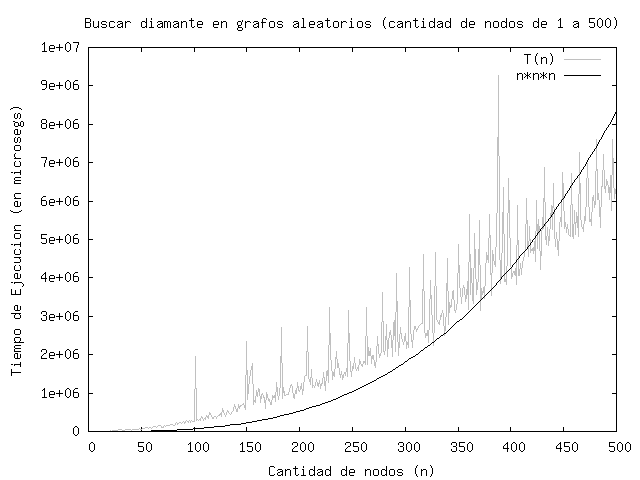
\includegraphics[width=0.7\textwidth]{Plots/Tp2Ej2-Complejidad.png}
\begin{center}
Figura 2.1
\end{center}
\end{center}

Como se puede apreciar en el gr\'afico, el crecimiento de los tiempos de ejecuci\'on del algoritmo es ligeramente inferior a la cota te\'orica propuesta. Como se mencion\'o anteriormente, esto se corresponde con lo esperado, ya que para este an\'alisis de utiliz\'o una cota mayor a la del algoritmo ($O(n^{3})$). Adem\'as se pueden apreciar irregularidades en la curva obtenida, lo que indica que el tiempo que se tarda en encontrar un diamante en un determinado grafo, adem\'as de depender de la cantidad de nodos, est\'a determinado por la disposici\'on de las aristas del mismo. Es decir, por la forma en la que est\'a hecho el algoritmo, el tiempo de ejecuci\'on va a depender de la cantidad de componentes conexas en las que tenga que buscar el diamante m\'inimo, para cada vecindad de cada nodo. Los peores casos se dar\'an en grafos en los que se busque un diamante en la mayor\'ia de las componentes conexas de cada vecindad. Estos casos hacen que las optimizaciones del algoritmo, que descartan la b\'usqueda de un diamante m\'inimo en ciertas componentes conexas, sean ineficientes. 

A continuaci\'on presentaremos alguno de estos casos ``patol\'ogicos'' y se ver\'a por qu\'e no se aplican las optimizaciones.

\begin{center}
 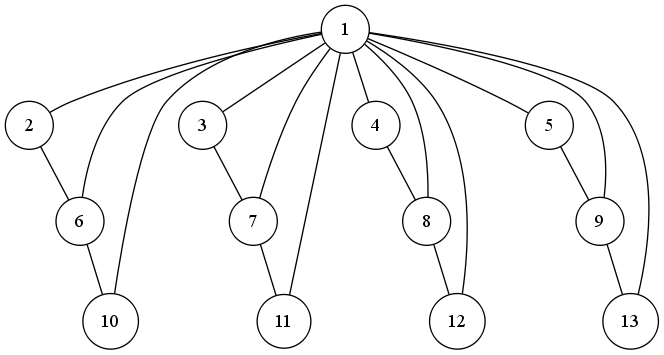
\includegraphics[width=0.7\textwidth]{Grafos/grafomati.png}
\begin{center}
Figura 2.2
\end{center}
\end{center}

Como se puede observar en el grafo presentado, la vecindad del nodo $1$ tiene varias componentes conexas que forman un diamante, ya que ninguna es completa. Por esta raz\'on, se deben estudiar todas las componentes conexas para encontrar el diamante m\'inimo. Sin embargo, podr\'ia darse el caso en que el algoritmo implementado no tenga que buscar el diamante m\'inimo para todas debido a que el m\'inimo nodo de una componente conexa (llamado nodoMinimoCompConexa en la secci\'on algoritmo) es menor que el m\'inimo nodo de las otras componentes. Esto suceder\'ia, por ejemplo, si el algoritmo comenzara a estudiar la componente conexa que comienza con el nodo $2$. Por el contrario, en el caso en que comenzara por la componente conexa que tiene el nodo $5$ y recorriera de derecha a izquierda las componentes conexas del gr\'afico, se tendr\'ia que calcular el m\'inimo diamante para todas las componentes, por lo que la cantidad de operaciones ser\'ia mayor. La forma en que se recorren las componentes conexas depende exclusivamente del orden de las listas de adyacencias pasadas como par\'ametro, por lo que la aparici\'on de estos peores casos estar\'a ligada a esta distribuci\'on. 

Cabe aclarar que el esquema presentado en la figura 2.2 representa s\'olo un caso simplificado sobre los peores casos que se pueden encontrar para el algoritmo mencionado. Es decir, en este gr\'afico s\'olo la vecindad del nodo $1$ podr\'ia representar un peor caso. F\'acilmente, este gr\'afico podr\'ia extenderse para formar casos a\'un peores, ya que cualquiera de las vecindades de los otros nodos podr\'ia tener las mismas dificultades que las del nodo $1$. Como los peores casos dependen del orden en que se reciben las listas de adyacencias, se hace dificultosa la b\'usqueda de los mismos. Por esta raz\'on, se opt\'o por explicar en detalle que representar\'ia un peor caso, ya que encontrar y hacer preubas de tiempo de ejecuci\'on sobre los mismos resultaba una tarea muy compleja.

\section*{Conclusiones}

En esta \'ultima secci\'on se realizar\'a una breve descripci\'on de los temas y resultados a tener en cuenta sobre este ejercicio. La primer parte del ejercicio requiri\'o un estudio profundo de teoria sobre subgrafos diamantes lo que permiti\'o una mayor facilidad para encarar la segunda parte y una buena cantidad de ideas a tener en cuenta. Sin embargo, el algoritmo presentado debi\'o encargarse de numerosas complicaciones que, a la hora de realizar la demostraci\'on de la propiedad referida al tema, no hab\'ian sido tenido en cuenta.

En mayor parte esto se debi\'o a la complejidad exigida por la c\'atedra lo que motiv\'o a la utilizaci\'on de distintas estructuras y m\'etodos (matrices y listas de adyacencia, estructuras de mapeo, algoritmos de busqueda inteligente, etc) que pudieran cumplir con lo pedido. Otro aspecto dificultoso fue el hecho de tener que retornar el diamante de menor tama\~{n}o, lo que implic\'o tener que guardar un registro de cada uno por componente conexa asociada a una vecindad, y no el primero en ser encontrado. Qued\'o a las claras aqu\'i como una idea que no es muy complicada ,como es la de encontrar un subgrafo inducido, puede volverse sumamente compleja al pedir ciertos requisitos sobre los resultados (en este caso el diamante m\'inimo).

En cuanto a las pruebas realizadas, estas arrojaron los resultados esperados en los casos en que se utilizaron grafos generados aleatoriamente. Tambi\'en hemos visto que para cierto tipo de grafos de entrada, puede que el algoritmo vari\'e notoriamente su tiempo de ejecuci\'on, a\'un asi cuando la cantidad de nodos es la misma. Esto se debe principalmente a dos razones. Una de ellas es la manera en que se construyen las listas de adyacencia utilizadas como estructura. Al no recibir los par\'ametros de entrada en orden, puede que el algoritmo obtenga primero los diamantes con nodos m\'as grandes, lo que no permitir\'ia evitar una gran cantidad de c\'alculos como si suceder\'ia en caso de obtener inicialmente los m\'inimos. El otro factor importante a tener en cuenta es el de la distribuci\'on de las aristas en el grafo, donde puede ocurrir que casi todas las componentes conexas de cada vecindad tengan la mayor cantidad de aristas pero sin ser completas. Esto implicar\'ia una gran cantidad de diamantes a buscar a comparaci\'on de casos promedio. Estos y otros casos patol\'ogicos son bastante complejos de generar sobre todo en grafos de gran tama\~{n}o por lo que su an\'alisis no pudo ser tan extenso como se dese\'o.

\begin{center}
\section*{Ejercicio 3: Red Astor}
\end{center}

\bigskip
\section*{Introducci\'on}

Básicamente, el enunciado del ejercicio propone resolver el problema de minimizar el costo de producción de una red ferroviaria que comunique distintos locales. Se sabe que cada vía tiene un costo de producción determinado y que existen ciertas vías fijas que deben ser incluidas en la solución. Sin demasiado esfuerzo, se observó que este problema se podría modelar como un problema de grafos de la siguiente manera: Cada nodo sería un local y las vias junto a su costo estarían representadas por cada arista. Como se trata de una red ferroviaria de menor costo producción, el problema a resolver es el de encontrar un árbol generador mínimo del grafo completo representado por cada local (nodo) considerando que ciertas aristas ya están prefijadas. Esto se debe a que en principio se podrían comunicar los locales de cualquier forma posible (grafo completo), se debe minimizar el costo (hallar aristas de menor peso) y es necesario que todo local esté comunicado y que exista un único camino entre ellos (es decir, un grafo conexo donde existe un único camino simple entre cada par de nodos, en otras palabras, un árbol).

Luego de modelado el problema, se procedió a idear una solución. De inmediato surgió la idea de utilizar un algoritmo similar a los vistos en clase que encuentran un árbol generador mínimo a partir de un grafo conexo ponderado cualquiera: Algortimo de Kruskal o Algoritmo de Prim. Debido a que el problema original plantea que ciertas aristas sean parte de la solución obligatoriamente, se evaluó si ambos algoritmos permitían encontrar dicho árbol aún partiendo de un conjunto de ejes ya establecidos. Rápidamente se descartó el algortimo de Prim ya que el mismo tiene como invariante que haya solamente una única componente conexa en cada paso por lo cual en caso de las aristas prefijadas no formen una única componente conexa dicho algoritmo no funcionará. Sin embargo, por la forma en la Kruskal se comporta funcionará aún cuando las aristas pasadas como parámetro formen más de una componente conexa como veremos más adelante.

En la sección siguiente veremos en detalle el algorimto propuesto junto con sus detalles implementativos.

\section*{Algoritmo}

Antes comenzar con el análisis, se presenta aqui el pseudocódigo que esboza la idea del algoritmo:

\begin{verbatim}
armarRed()
  aristasPorAgregar = lista de aristas del grafo original
  aristasAstor = lista de aristas prefijadas por Astor
  ordenar aristasPorAgregar por peso

  insertar aristasAstor en el grafo resultado
  costoProduccion = sumo los pesos de todas las aristas de astor

  mientras la cantidad agregada sea menor a n-1 nodos
    tomo una arista de aristasPorAgregar
    si se puede insertar la arista (sePuedeMeter)
      sumar a costoProduccion el peso de la arista
      insertar la arista en el grafo resultado (meterArista)

  ordenar las aristas del grafo resultado segun los valores de los nodos

sePuedeMeter(arista)
  si los dos nodos distintas a la misma componente conexa 
  o si alguno de los dos no pertenece a ninguna
    retornar true
  sino
    retornar false

meterArista(arista)
  si ninguno de los dos nodos pertenece a alguna componente conexa
    asignar una nueva componente conexa a ambos nodos

  sino si un nodo pertenece a alguna componente y el otro no
    asignar al otro nodo esa componente

  sino si ambos nodos pertenecen a componentes conexas distintas
    uno las dos componentes en una y le asigno a ambos nodos esa componente

  agrego la arista al grafo resultante
\end{verbatim}

En primer lugar, como se puede observar, \textit{armarRed()} es la función principal del algoritmo encargada de generar el arbol generador mínimo del grafo (con aristas prefijadas), es decir, armar la red ferroviaria. Como se mencionó, este algorimto es básicamente el algoritmo de Kruskal para armar el árbol generador mínimo con algunas particularidades. El primer procedimiento consiste en almacenar las aristas prefijadas por Astor y las aristas para agregar en listas enlazadas. Luego se ordenan las aristas a agregar de menor a mayor mediante un algoritmo de sorting eficiente (basado en \textit{Quicksort}) provisto por las librerías del lenguaje, con el fin de poder luego tomar cada arista mínima en cada paso en tiempo constante. Finalmente, el ciclo principal se encarga se armar el árbol resultado de la siguiente manera: Toma una arista de la lista (la mínima hasta ese paso) y pregunta si se puede insertar (\textit{sePuedeMeter()}), es decir si no formará un ciclo que rompa con el invariante de árbol. En caso afirmativo, inserta la arista al grafo (\textit{meterArista()}), acomodando las estructuras como veremos a continuación. Caso contrario, descarta la arista y prosigue con la siguiente, hasta haber insertado $n-1$ aristas, es decir, haber formado el árbol.

Probablemente el aspecto más interesante a analizar de este algoritmo sean las formas de verficación de ciclo y las estructuras asociadas a estos procedimientos. Razonando, se llegó a la conclusión que verificar la existencia de un ciclo en el árbol al insertar una arista equivale a observar a que componente conexa pertenece cada nodo de la arista en cuestión. En caso de pertenecer ambos nodos a la misma componente conexa es porque la arista formará un ciclo y debe ser descartada. Por este motivo, se concluyó que lo ideal sería encontrar una estructura que permita asociar cada nodo a una componente conexa, permitiendo verificar esto de manera eficiente. Abstrayéndose de esta cuestión, se notó que se debería contar con una estrucutura que represente a varios conjuntos disjuntos, uno por cada componente conexa, que logre buscar a que conjunto pertenece un determinado elemento (nodo) y que consiga unir dos conjuntos en forma óptima. Razonando más profundamente, se llegó a la conclusión de que no se podía obtener una estructura que permita realizar ambas operaciones en tiempo constante: si se podía ver la pertenencia en forma constante, la union tomaría tiempo de orden lineal y viceversa. Como la unión se realiza en ciertos casos (al hallar una arista cuyos nodos pertenezcan ya a distintas componentes conexas) mientras que la busqueda es obligada en cada iteración (para verificar si hay ciclo) se optó por priorizar esta última.

Las estructuras elegidas para respresentar a las componentes conexas (conjuntos disjuntos) fueron dos arreglos de igual tamaño (cantidad de nodos/locales): \textit{índices} y \textit{componentesConexas}. Para el primero de ellos (\textit{índices}), cada posición representa un nodo de ese valor mientras que su contenido es alguna posición del segundo arreglo (\textit{componentesConexas}). Este último contiene un número que representa una componente conexa. Ambos arreglos comienzan con todas sus posiciones en $0$ (los nodos no pertenecen a ninguna componente conexa, ya que ninguna arista fue insertada). De esta forma las funciones \textit{sePuedeMeter()} y \textit{meterArista()} se encagarán de observar y modificar estas estructuras, respectivamente.

Con estas estructuras, verificar si hay ciclo (\textit{sePuedeMeter()}) radica simplemente en ir a la posición del arreglo \textit{índices} para ambos nodos y luego acceder al arreglo \textit{componentesConexas} para comprobar si esas posiciones hacen referencia las mismas componentes conexas. De este modo, la operacion de búsqueda se realiza en tiempo constante.

La función \textit{meterArista()} se encargará de acomodar la estructura para mantener la coherencia. De acuerdo a los nodos de la arista en cuestión, tal como se puede ver en el pseudocódigo, existen 3 casos:
\begin{itemize}
 \item \textbf{Los nodos no pertenecen a ninguna componente conexa:} En este caso, para cada posición de ambos nodos se asigna un nuevo valor de componente conexa (contador \textit{compConexaActual}) al arreglo de \textit{índices}. Luego, en la posición \textit{compConexaActual} del arreglo \textit{componentesConexas} se guarda ese mismo valor. Finalmente, se incrementa el contador \textit{compConexaActual} de componentes conexas.

 \item \textbf{Un nodo pertenece a alguna componente conexa y el otro no:} Simplemente se actualiza la posición del nodo que no pertenecía a ninguna componente conexa en el arreglo \textit{índices} con el valor de la componente conexa del otro nodo (que si se encontrada en alguna componente conexa).

 \item \textbf{Los nodos pertenecen a componentes conexas distintas:} Este último caso es el más costoso, ya que es en el cuál se debe realizar la unión de las componentes conexas a las que pertencen cada uno de los dos nodos. Para realizar esto, se recorre el arreglo \textit{componentesConexas} y por cada elemento que pertenecía a la componente conexa del segundo nodo se le asigna el número de componente conexa del primer nodo.
\end{itemize}

De este modo, la función \textit{meterArista()} logra mantener la consistencia en todos los casos posibles de forma de que \textit{sePuedeMeter()} retorne siempre los valores esperados.

Concluido el cicilo, se habrán insertado las $n-1$ aristas necesarias para generar el árbol de forma que no haya ciclos logrando así el objetivo propuesto. Finalmente, a fines de cumplir con lo pedido, se ordenan las aristas según los valores de cada nodo.

Con respecto a la utilización de otras estructuras para mejorar la complejidad, se investigó acerca del asunto, concluyendo efectivamente que no se podrían encontrar formas de resolver el problema de los conjuntos disjuntos de una manera \textit{asintóticamente} mejor. Sin embargo, como veremos en la sección ``Conclusiones``, existen formas de optimizar las estructuras y los algorimos propuestos.

\section*{Correctitud}

A continuaci\'on se presentar\'a la demostraci\'on de correctitud del algoritmo implementado. Dividiremos la demostraci\'on en dos partes. Primero mostraremos que el grafo que retorna el algoritmo es un \'arbol generador del grafo recibido como par\'ametro. Luego veremos que ademas dicho \'abrol generador es m\'inimo.

Vale aclarar que las aristas agregadas en el primer ciclo del algoritmo (las aristas elegidas por Astor) nunca pueden formar un ciclo por precondici\'on.

Sea $G$ el grafo recibido como par\'ametro y $T$ el grafo resultado de aplicar \textit{armarRed}:

\begin{itemize}
\item $T$ es \'arbol generador de $G$

Para comenzar, mostraremos que $T$ es conexo. Supongamos entonces que no lo es para llegar a un absurdo. Sea $e$ una arista de $G$ que une dos componentes conexas distintas de $T$. Dicha arista debi\'o ser considerada en algun paso del algoritmo como una posible arista para agregar a $T$. Como todas las aristas que no formen un ciclo son agregadas en cada paso del algoritmo, es absurdo que $e$ no pertenezca a $T$, puesto que si en el grafo final $e$ une dos componentes conexas de $T$, es decir que no forma ciclo en $T$, tampoco hubiese formado un ciclo en el momento en el que fue considerada para ser insertada ya que nunca se remueven aristas.

Trivialmente se puede apreciar que $T$ es ac\'iclico, puesto que no se agrega ninguna arista que forme un ciclo. Adem\'as es tambi\'en trivial que $T$ contiene todos los nodos de $G$ (se agregan $n-1$ aristas que no forman ciclos).

De esta manera podemos concluir que $T$ es un \'arbol generador m\'inimo de $G$, puesto que contiene todos los nodos de $G$, es conexo y no posee ciclos. Cabe mencionar que si la cantidad de aristas que se colocan sin chequeos por la elecci\'on de Astor es igual a $n-1$ entonces no se recorer\'a el segundo ciclo para agregar aristas porque por precondici\'on ya tendr\'ia formado mi \'arbol generador.

\item $T$ es \'arbol generador que contiene las aristas prefijadas m\'inimo de $G$

Nuevamente encararemos esta demostraci\'on por el absurdo. Supongamos entonces que $T$ es \'arbol generador (conteniendo las aristas de Astor) no m\'inimo de $G$ y que existe un grafo $S$ distinto de $T$ que si lo es. Sea $e$ la primer arista elegida por el algoritmo que pertenece a $T$ pero no a $S$. Como $e$ no pertenece a $S$, entonces si a $S$ le agrego la arista $e$ (notado $S+e$) $S+e$ contendr\'a un ciclo. Adem\'as existe $e'$ perteneciente al ciclo formado en $S$ tal que $e'$ no pertenece a $T$. Esto sucede porque si $e'$ perteneciera a $T$ entonces tendria un ciclo lo que es absurdo porque es \'arbol:

\begin{center}
 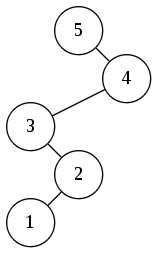
\includegraphics[width=0.22\textwidth]{Grafos/ej3figura1.png}
\hspace{100pt}
 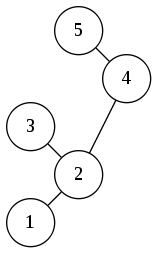
\includegraphics[width=0.22\textwidth]{Grafos/ej3figura2.png}
\begin{center}
 Grafo $T$ \hspace{160pt} Grafo $S$
\end{center}
\end{center}

En el ejemplo mostrado $e$ ser\'ia la arista (3,4) y $e'$ ser\'ia (2,4). Sea $S'=S+e-e'$, de esta manera $S'$ es \'arbol generador de $G$. Si $l(e')<l(e)$ ($l(e)=$ peso de la arista $e$) llego a un absurdo. Esto se puede ver porque $S$ contiene todas las aristas anteriores a $e$ m\'as $e'$ y no se forma un ciclo en dicho grafo, por consiguente el algoritmo que va armando el grafo $T$ hubiese elegido a $e'$ en lugar de $e$ y esto es absurdo porque dijimos que $e'$ no pertenece a $T$. Entonces tenemos que $l(e')\geq l(e)$. Podemos apreciar entonces que el peso de $S'$ es a lo sumo igual al de $S$, pero no puede ser menor porque $S$ es AGM. Esto implica que $S'$ tiene el mismo peso que $S$ y entonces tambien es \'arbol generador m\'inimo de $G$ (conteniendo las aristas prefijadas), m\'as a\'un, $S'$ tiene una arista m\'as en com\'un con $T$ que $S$. Repitiendo este paso para todas las aristas distintas entre $T$ y $S$ (como m\'aximo ser\'an $l-f-1$ pasos, donde $l$ es la cantidad de nodos y $f$ la cantidad de pares fijados por Astor), se llegar\'a a un grafo \'arbol generador m\'inimo de $G$ con las mismas aristas de $T$, lo que es absurdo porque partimos de que $T$ no es m\'inimo.

\end{itemize}

\section*{Complejidad}

\textbf{TODO}

\section*{An\'alisis de resultados}

En la siguiente secci\'on analizaremos el comportamiento en la pr\'actica del algoritmo propuesto. El an\'alisis est\'a basado en estudiar el tiempo de ejecuci\'on para instancias aleatorias en funci\'on de la cantidad de locales manteniendo fija la cantidad de pares de locales fijados por Astor es decir, seg\'un el modelo propuesto, la cantidad de aristas a ingresar en el \'arbol antes de iniciar el algoritmo. A su vez, se ver\'a la relaci\'on que existe entre la complejidad te\'orica calculada y los resultados obtenidos. Adem\'as, para completar el an\'alisis se estudiar\'an los peores casos que presenta el algoritmo.

Para realizar los tiempos de ejecuci\'on, se implement\'o un algoritmo que genera instancias aleatorias, es decir, genera la matriz de los pesos de cada arista para todo el grafo completo y una cierta cantidad de aristas, que representan los locales fijados por Astor, asegur\'andose que no formen un ciclo.

A continuaci\'on se presentan los resultados de las pruebas realizadas para instancias aleatorias, variando la cantidad de locales y manteniendo fija la cantidad de pares fijado por Astor en $4$, $20$ y $50$.

\begin{center}
 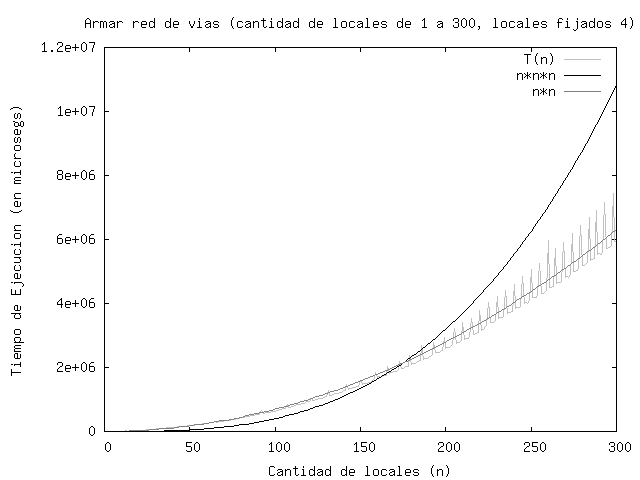
\includegraphics[width=0.7\textwidth]{Plots/Tp2Ej3-Complejidad.png}
\begin{center}
Figura 3.1
\end{center}
\end{center}

\begin{center}
 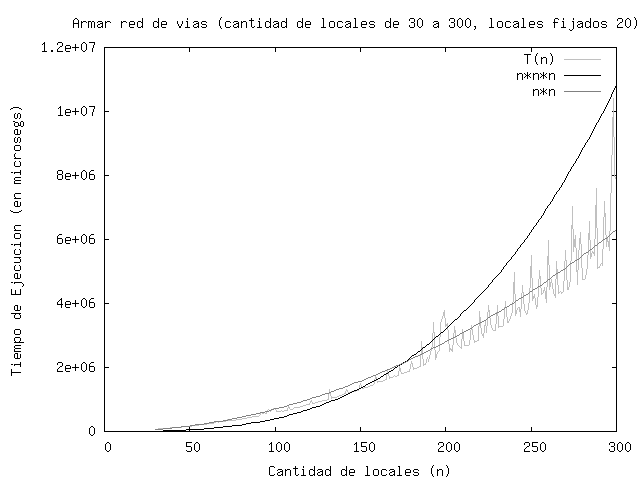
\includegraphics[width=0.7\textwidth]{Plots/Tp2Ej3-Complejidad-20.png}
\begin{center}
Figura 3.2
\end{center}
\end{center}

\begin{center}
 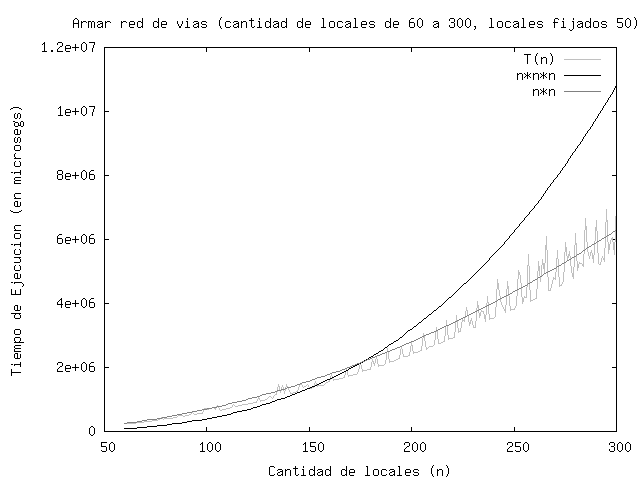
\includegraphics[width=0.7\textwidth]{Plots/Tp2Ej3-Complejidad-50.png}
\begin{center}
Figura 3.3
\end{center}
\end{center}

Como se puede apreciar, en las figuras $3.1$, $3.2$ y $3.3$ el crecimiento de la funci\'on que mide el tiempo de ejercuci\'on es similar, a pesar de que, a mayor cantidad de locales fijados por Astor, los tiempos se vuelven m\'as irregulares. La similitud en el crecimiento de los gr\'aficos se debe a que el tiempo que tarda algoritmo depende sobre todo de la disposici\'on de las aristas fijadas por Astor y de la forma en que se van agregando las aristas durante el algoritmo de Kruskal, y no tanto de la cantidad de aristas recibidas. Es decir, si se mantiene fija la cantidad de aristas de Astor y se aumenta significativamente la cantidad de locales totales, la incidencia de este par\'ametro en el tiempo de ejecuci\'on ser\'a m\'inima.

Es importante observar que en las figuras presentadas el crecimiento de la funci\'on del tiempo de ejecuci\'on es menor que la cota te\'orica propuesta, $O(n^{3})$. El gr\'afico muestra adem\'as que dicho crecimiento se asemeja mucho m\'as al orden cuadr\'atico. Esto se debe a la forma en que el algoritmo arma el \'arbol resultante: la mayor\'ia de las aristas que agrega en los sucesivos pasos del algoritmo de Kruskal, se agregan en tiempo constante. Agregar una arista es de orden lineal s\'olo en el caso en que dicha arista une dos componentes conexas del \'arbol, es decir, cuando se deben recorrer las estructuras utilizadas para cambiar una de las componentes conexas fusionadas. Sin embargo, emp\'iricamente esta \'ultima operaci\'on  se realiza pocas veces en relaci\'on a la cantidad total de aristas agregadas. Por esta raz\'on, en el caso promedio la complejidad del algoritmo es menor que la cota te\'orica propuesta de $O(n^{3})$. Por medio de las pruebas, podr\'iamos afirmar entonces que en la pr\'actica el algoritmo presentado se asemeja m\'as a un algoritmo de orden cuadr\'atico que a uno c\'ubico.

Seg\'un lo mencionado anteriormente, se puede deducir que los peores casos ser\'an aquellos en los que agregar una arista al \'arbol resultado implique unir componentes conexas y, por lo tanto, tener que cambiar la estructura que guarda el n\'umero de componente conexa de cada nodo (llamada ComponentesConexas en la secci\'on ``Algoritmo``). A continuaci\'on presentaremos un ejemplo de peor caso y lo explicaremos en detalle.

\begin{center}
 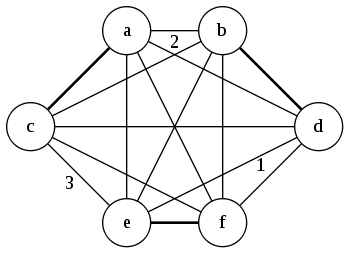
\includegraphics[width=0.6\textwidth]{Grafos/ej3peorcaso.png}
\begin{center}
Figura 3.4
\end{center}
\end{center}

En primer lugar, se deben hacer ciertas aclaraciones: 
\begin{itemize}
 \item Las aristas fijadas por Astor son las que figuran resaltadas.
 \item El peso de las aristas del ''interior del grafo'' es mayor que las del ``borde``.
\end{itemize}

Como se puede notar en el gr\'afico, la arista de menor peso es la $D-F$ por lo que ser\'a la primera en ser agregada en el algoritmo. Agregar esta arista implica unir las componentes conexas de las aristas $E-F$ y $D-B$, por lo que se deber\'a recorrer todo el arreglo ComponentesConexas para eliminar las apariciones de la componente conexa $D-B$ y as\'i fusionar las tres aristas mencionadas en una \'unica componente conexa que contenga a los nodos E, F, D, B. Esta misma operaci\'on se realizar\'a para unir esta \'ultima componente conexa con la componente que contiene a los nodos C y A por medio de la arista $A-B$. En este caso, todas las aristas agregadas unieron componentes conexas, por lo que se debi\'o recorrer el arreglo ComponentesConexas por cada arista haciendo que este sea un peor caso para el algoritmo presentado. Cabe aclarar que estos casos dependen tanto de la disposici\'on tanto de las aristas de Astor, como del peso de las aristas a agregar. Esto hace que generar peores casos para estudiar el tiempo de ejecuci\'on sea d\'ificil. Sin embargo, seg\'un el ejemplo presentado y la cota te\'orica propuesta se puede apreciar que el tiempo de los peores casos ser\'a del orden de $n^{3}$.

\section*{Conclusiones}

A partir de las secciones detalladas anteriormente se pueden realizar las siguientes conclusiones y aclaraciones. En primer lugar, es importante aclarar que a la hora de resolver el problema se podr\'ian haber utilizado otro tipo de estructuras para mejorar el rendimiento del algoritmo. Como el algoritmo propuesto se basa principalmente en hacer operaciones de bu\'squeda y uni\'on sobre distintos conjuntos de nodos, se podr\'ia haber utilizado una estructura \textit{Union-Find}\footnotemark[1]. En la pr\'actica este tipo de estructuras hacen que el algoritmo mejore significativamente su complejidad debido a que las operaciones de uni\'on y b\'usqueda son pr\'acticamente lineales (utilizando algoritmos inteligentes sobre listas y \'arboles). Cabe aclarar que a pesar de esto la cota te\'orica es la misma que se obtiene con las estructuras utilizadas en nuestro algoritmo.

Como se pudo observar emp\'iricamente, llegamos a la conclusi\'on de que el algoritmo es mejor en promedio de lo que se esperaba en teor\'ia. Es decir, se mostr\'o que tiene un comportamiento del orden cuadr\'atico para la mayor\'ia de los casos, aunque existen casos en lo que esto no es cierto. Cabe mencionar tambi\'en que se podr\'ian haber hecho otras pruebas para estudiar el comportamiento del algoritmo. En concreto, se podr\'ia haber hecho un an\'alisis de los tiempos de ejecuci\'on en funci\'on de la cantidad de aristas de Astor, manteniendo fija la cantidad de locales. Se supone que a medida que aumente la cantidad de aristas de Astor para una cantidad de locales fija, el tiempo de ejecuci\'on deber\'ia disminuir ya que debe agregar menor cantidad de aristas teniendo que chequear si se forma un ciclo.

Finalmente, podemos concluir que el problema podr\'ia haber sido resuelto de manera un poco m\'as eficiente de haber tenido tiempo adicional. Sin embargo, en la pr\'actica, el tiempo de ejecuci\'on del algoritmo propuesto se asemeja m\'as al de los algoritmos que utilizan \textit{Union-Find} que a un algoritmo de orden c\'ubico.

\footnotetext[1]{Ver referencias sobre este tipo de estructuras en la secci\'on ''Referencias''}

\section*{Referencias}
\begin{itemize}
 \item Art\'iculo de Wikipedia sobre Programaci\'on Din\'amica
 \item Art\'iculo de Wikipedia sobre Grafos
 \item Art\'iculo de Wikipedia sobre Algoritmo de Kruskal
 \item Art\'iculo de Wikipedia sobre Estructuras Union-Find
 \item Art\'iculo de Wikipedia sobre Depth/Breadth First Search
\end{itemize}


\end{document}
